\documentclass[12pt]{article}
\usepackage{amsmath, amssymb, amsthm, tikz, pgfplots}
\usepackage{geometry, enumitem, mdframed, array, xcolor}
\geometry{margin=1in}

% Custom environments
\newtheorem{definition}{Definition}
\newtheorem{theorem}{Theorem}
\newtheorem{method}{Method}
\newtheorem{example}{Example}
\newmdenv[linecolor=blue,linewidth=2pt]{keypoint}
\newmdenv[linecolor=red,linewidth=2pt]{warning}
\newmdenv[linecolor=green,linewidth=2pt]{insight}
\newmdenv[linecolor=purple,linewidth=2pt]{examtip}
\newmdenv[linecolor=cyan,linewidth=2pt]{algorithm}

\title{ODE Lesson 25: Orthogonal Trajectories and Applications}
\author{ODE 1 - Prof. Adi Ditkowski}
\date{}

\begin{document}
\maketitle

\section{Definition and Geometric Interpretation}

\begin{definition}[Orthogonal Trajectories]
Given a one-parameter family of curves $F(x,y,c) = 0$, the \textbf{orthogonal trajectories} are curves that intersect each member of the family at right angles (90°).
\end{definition}

\begin{keypoint}
At any point of intersection, the product of the slopes of two orthogonal curves equals $-1$:
\[m_{1} \cdot m_{2} = -1\]
This is the fundamental principle behind finding orthogonal trajectories.
\end{keypoint}

\section{The Systematic Method}

\begin{algorithm}
\textbf{Finding Orthogonal Trajectories:}
\begin{enumerate}
    \item Start with family $F(x,y,c) = 0$
    \item Differentiate to eliminate parameter $c$:
    \[\frac{\partial F}{\partial x} + \frac{\partial F}{\partial y}\frac{dy}{dx} = 0\]
    \item Express as differential equation: $\frac{dy}{dx} = f(x,y)$
    \item Replace $\frac{dy}{dx}$ with $-\frac{dx}{dy}$ to get orthogonal equation:
    \[-\frac{dx}{dy} = f(x,y)\]
    \item Solve the new differential equation
    \item The solution gives the orthogonal trajectories
\end{enumerate}
\end{algorithm}

\begin{warning}
You MUST eliminate the parameter $c$ before forming the differential equation. Failing to do so is the most common error and leads to incorrect results!
\end{warning}

\section{Classic Examples}

\begin{example}[Straight Lines Through Origin]
Find orthogonal trajectories of $y = cx$.

\textbf{Solution:}
\begin{enumerate}
    \item Differentiate: $\frac{dy}{dx} = c$
    \item Eliminate $c$: Since $c = \frac{y}{x}$, we have $\frac{dy}{dx} = \frac{y}{x}$
    \item Orthogonal equation: $-\frac{dx}{dy} = \frac{y}{x}$ or $\frac{dx}{dy} = -\frac{y}{x}$
    \item Rearrange: $x dx = -y dy$
    \item Integrate: $\frac{x^{2}}{2} = -\frac{y^{2}}{2} + C$
    \item Simplify: $x^{2} + y^{2} = K
\end{enumerate}
The orthogonal trajectories are circles centered at the origin!
\end{example}

\begin{example}[Exponential Curves]
Find orthogonal trajectories of y = ce^{2x}.

\textbf{Solution:}
\begin{enumerate}
    \item Differentiate: \frac{dy}{dx} = 2ce^{2x}
    \item Eliminate c: From original, c = ye^{-2x}, so \frac{dy}{dx} = 2y
    \item Orthogonal equation: $-\frac{dx}{dy} = 2y$ or $\frac{dx}{dy} = -2y$
    \item Integrate: $x = -y^{2} + C$
    \item Result: $x + y^{2} = K$ (parabolas opening left)
\end{enumerate}
\end{example}

\section{Visualization of Orthogonal Families}

\begin{center}
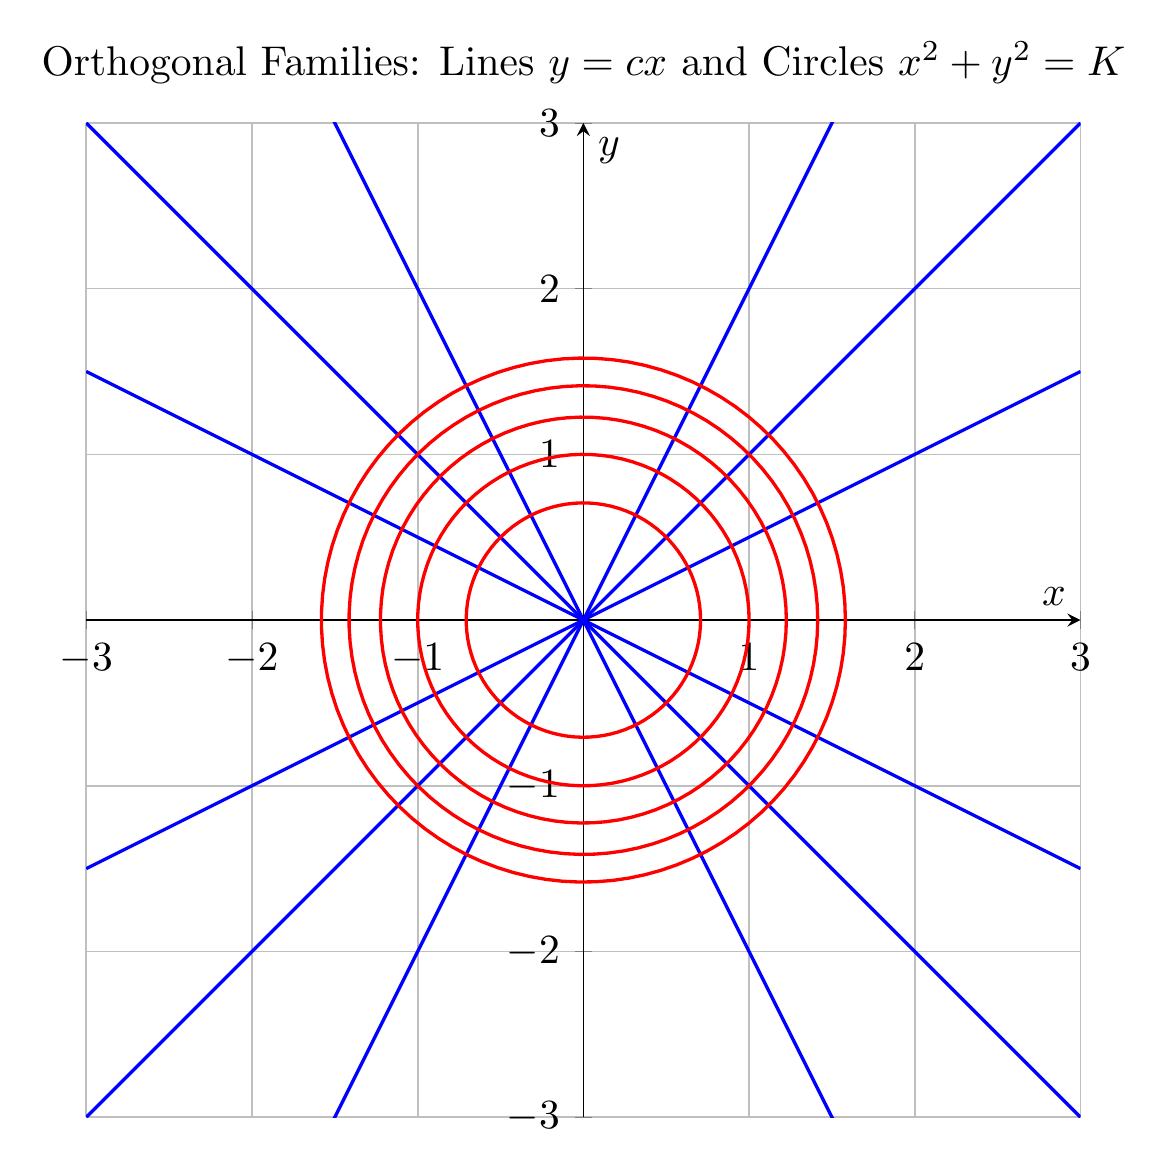
\begin{tikzpicture}[scale=1.5]
\begin{axis}[
    axis lines = center,
    xlabel = $x$,
    ylabel = $y$,
    xmin=-3, xmax=3,
    ymin=-3, ymax=3,
    title={Orthogonal Families: Lines $y=cx$ and Circles $x^{2}+y^{2}=K$},
    grid=major,
    width=10cm,
    height=10cm
]

% Draw lines y = cx
\foreach \c in {-2,-1,-0.5,0.5,1,2} {
    \addplot[blue, thick, domain=-3:3, samples=2] {x*\c};
}

% Draw circles x^{2} + y^{2} = K
\foreach \k in {0.5,1,1.5,2,2.5} {
    \addplot[red, thick, domain=0:360, samples=100, parametric]
    ({sqrt(\k)*cos(x)},{sqrt(\k)*sin(x)});
}

\end{axis}
\end{tikzpicture}
\end{center}

\section{Self-Orthogonal Families}

\begin{definition}[Self-Orthogonal]
A family of curves is \textbf{self-orthogonal} if its orthogonal trajectories belong to the same family (with different parameter values).
\end{definition}

\begin{example}[Rectangular Hyperbolas]
The family $xy = c$ is self-orthogonal.

\textbf{Proof:}
\begin{enumerate}
    \item Differentiate: $y + x\frac{dy}{dx} = 0$, so $\frac{dy}{dx} = -\frac{y}{x}$
    \item Orthogonal equation: $-\frac{dx}{dy} = -\frac{y}{x}$ or $\frac{dx}{dy} = \frac{y}{x}$
    \item Rearrange: $\frac{x dx}{y dy} = 1$, so $x dx = y dy$
    \item Integrate: $\frac{x^{2}}{2} = \frac{y^{2}}{2} + C$
    \item This gives $x^{2} - y^{2} = K$, or $(x-y)(x+y) = K$
\end{enumerate}
Actually, more careful analysis shows these are also rectangular hyperbolas, rotated by 45°.
\end{example}

\section{Physical Applications}

\begin{keypoint}
\textbf{Orthogonal Trajectories in Physics:}
\begin{center}
\begin{tabular}{|l|l|l|}
\hline
\textbf{Field} & \textbf{Family 1} & \textbf{Family 2 (Orthogonal)} \\
\hline
Electrostatics & Electric field lines & Equipotential surfaces \\
Fluid Dynamics & Streamlines & Velocity potential lines \\
Heat Transfer & Heat flow lines & Isotherms (constant temperature) \\
Magnetism & Magnetic field lines & Constant flux surfaces \\
Stress Analysis & Principal stress trajectories & Shear stress trajectories \\
\hline
\end{tabular}
\end{center}
\end{keypoint}

\begin{insight}
The orthogonality of field lines and equipotentials follows from the fact that the gradient (field) is perpendicular to level curves (equipotentials). This is why $\vec{E} = -\nabla V$.
\end{insight}

\section{Polar Coordinate Form}

\begin{theorem}[Orthogonal Trajectories in Polar Coordinates]
If a family of curves in polar coordinates satisfies the differential equation
\[\frac{dr}{d\theta} = F(r,\theta)\]
then the orthogonal trajectories satisfy
\[r^{2}\frac{d\theta}{dr} = F(r,\theta)\]
\end{theorem}

\begin{example}[Cardioids]
Find orthogonal trajectories of $r = a(1 + \cos\theta)$ (family of cardioids).

The differential equation and solution involve more complex polar calculus, but the principle remains: multiply by $r^{2}$ and interchange the roles of $r$ and $\theta$ derivatives.
\end{example}

\section{Connection to Complex Analysis}

\begin{theorem}[Cauchy-Riemann and Orthogonality]
If $f(z) = u(x,y) + iv(x,y)$ is analytic, then the families $u(x,y) = c_{1}$ and $v(x,y) = c_{2}$ are orthogonal trajectories.
\end{theorem}

\begin{example}[Complex Function]
For $f(z) = z^{2} = (x+iy)^{2} = x^{2} - y^{2} + 2ixy$:
\begin{itemize}
    \item Real part: $u = x^{2} - y^{2} = c_{1}$ (hyperbolas)
    \item Imaginary part: $v = 2xy = c_{2}$ (hyperbolas)
    \item These families are orthogonal!
\end{itemize}
\end{example}

\section{Common Exam Patterns}

\begin{examtip}
Prof. Ditkowski's favorite orthogonal trajectory problems:
\begin{enumerate}
    \item Circles and radial lines: $x^{2} + y^{2} = c^{2}$ ↔ $y = kx$
    \item Parabolas and exponentials: $y^{2} = cx ↔ y = ke^{2x}
    \item Confocal ellipses and hyperbolas (advanced)
    \item Temperature distribution and heat flow
    \item Self-orthogonal families (always one question!)
\end{enumerate}
\end{examtip}

\section{Step-by-Step Strategy}

\begin{algorithm}
\textbf{Exam Problem Approach:}
\begin{enumerate}
    \item Identify the given family F(x,y,c) = 0
    \item Differentiate with respect to $x$ (implicit differentiation if needed)
    \item Eliminate parameter $c$ using the original equation
    \item Write differential equation: $\frac{dy}{dx} = f(x,y)$
    \item Form orthogonal equation: $\frac{dx}{dy} = -f(x,y)$
    \item Solve (may require exact equations or integrating factors!)
    \item Verify orthogonality by checking slopes at intersection points
    \item Sketch both families showing perpendicular intersections
\end{enumerate}
\end{algorithm}

\end{document}